
%(BEGIN_QUESTION)
% Copyright 2006, Tony R. Kuphaldt, released under the Creative Commons Attribution License (v 1.0)
% This means you may do almost anything with this work of mine, so long as you give me proper credit

Qualitatively graph the response of an hypothetical derivative-only controller over time to the following changes in process variable:

$$\includegraphics[width=15.5cm]{i01537x01.eps}$$

Assume {\it reverse} control action.
 
\underbar{file i01537}
%(END_QUESTION)





%(BEGIN_ANSWER)

The controller output graph shown here is {\it qualitative} only.  Although drawn to scale (i.e. all changes in the output are properly scaled relative to each other), the scale itself is arbitrary and therefore may not match the scale of your sketch:

$$\includegraphics[width=15.5cm]{i01537x02.eps}$$

Derivative action looks only at the {\it rate-of-change} of the error signal.  In this case, since the SP is constant, derivative acts only on the PV's {\it slope}.  During the time period where the PV rises 15\% over a run (time span) of 6 units, I plot the output as a constant 5\% below the original output signal value (from 32.5\% to 27.5\%).  When the PV falls the same amount (15\%) over the same time span, the output goes to a value 5\% above the original value (from 32.5\% to 37.5\%).

When the PV begins to fall at a faster rate (20\% in 2 units), the rise/run slope ratio is 4 times as much as before.  Thus, the output goes to a value 4 times as great as before (20\% instead of 5\%), from 32.5\% to 52.5\%.  When the PV returns to SP at the same (steep) rate, the output drops 20\% below the original starting value (from 32.5\% to 12.5\%).
%(END_ANSWER)





%(BEGIN_NOTES)


%INDEX% Control, derivative: graphing controller response

%(END_NOTES)


